\documentclass{beamer}
\usepackage{graphicx}
\usetheme{Warsaw}
\graphicspath{{C:/Projects/urban-design/resources/}}

\begin{document}

    \title{Urban design}
    \author{Vasily Ermakov}
    \date{Vilnius, 2022}
    \frame{\titlepage}

    \begin{frame}{Stroad}
        \begin{block}
            <+->{Portmanteau}
            \textbf{Portmanteau} is a word blending the sounds and combining the meanings of two others.\\
            \begin{itemize}
                \item smog = smoke + fog
                \item cosplay = costume + play
                \item sitcom = situational + comedy
            \end{itemize}
        \end{block}
        \begin{block}
            <+->{}
            What \textbf{stroad} could be blend of?
        \end{block}
        \begin{block}
            <+->{}
            \begin{itemize}
                \item stroad = street + road
            \end{itemize}
        \end{block}
    \end{frame}

    \begin{frame}{Stroad}
        \begin{block}
            <+->{}
            What are the differences between street and road?
        \end{block}
        \begin{block}
            <+->{Road}
            \begin{itemize}
                \item High-speed connection
                \item Wide lanes
                \item Straight
                \item Gentle curves
                \item Clear zone
                \item Large signs
                \item Fewer entrances \& exits
            \end{itemize}
        \end{block}
    \end{frame}

    \begin{frame}{Stroad}
        \begin{block}
            <+->{Street}
            \begin{itemize}
                \item Complex environment where life in the city happens
                \item Buildings are placed right to sidewalk \& are easily accessible by pedestrians.
                \item Comfortable place to be in
                \item Many entrances \& exits
                \item Street parking
                \item Low speeds
                \item Walkable
            \end{itemize}
        \end{block}
        \begin{block}
            <+->{Stroad}
            \begin{itemize}
                \item Changing lanes, going in \& out slows down traffic and creates many points of conflict. Drivers are slowing down to avoid collision.
                \item Dangerous for people walking \& cycling
            \end{itemize}
        \end{block}
    \end{frame}

    \begin{frame}{Dzerzhinsky avenue, Minsk}
        \includegraphics[width = \textwidth]{Dzerzhinsky avenue.PNG}
    \end{frame}

    \begin{frame}{Dzerzhinsky avenue, Minsk}
        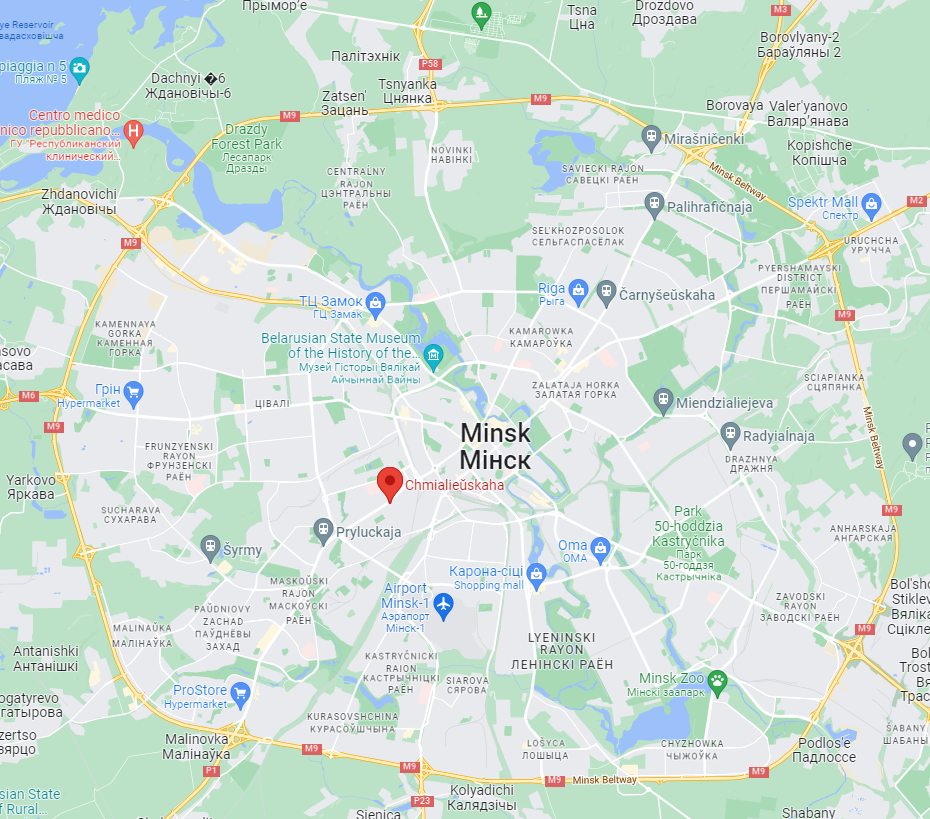
\includegraphics[width = 0.8\textwidth]{Dzerzhinsky avenue map.PNG}
    \end{frame}

    \begin{frame}{Einsteinweg, Amsterdam}
        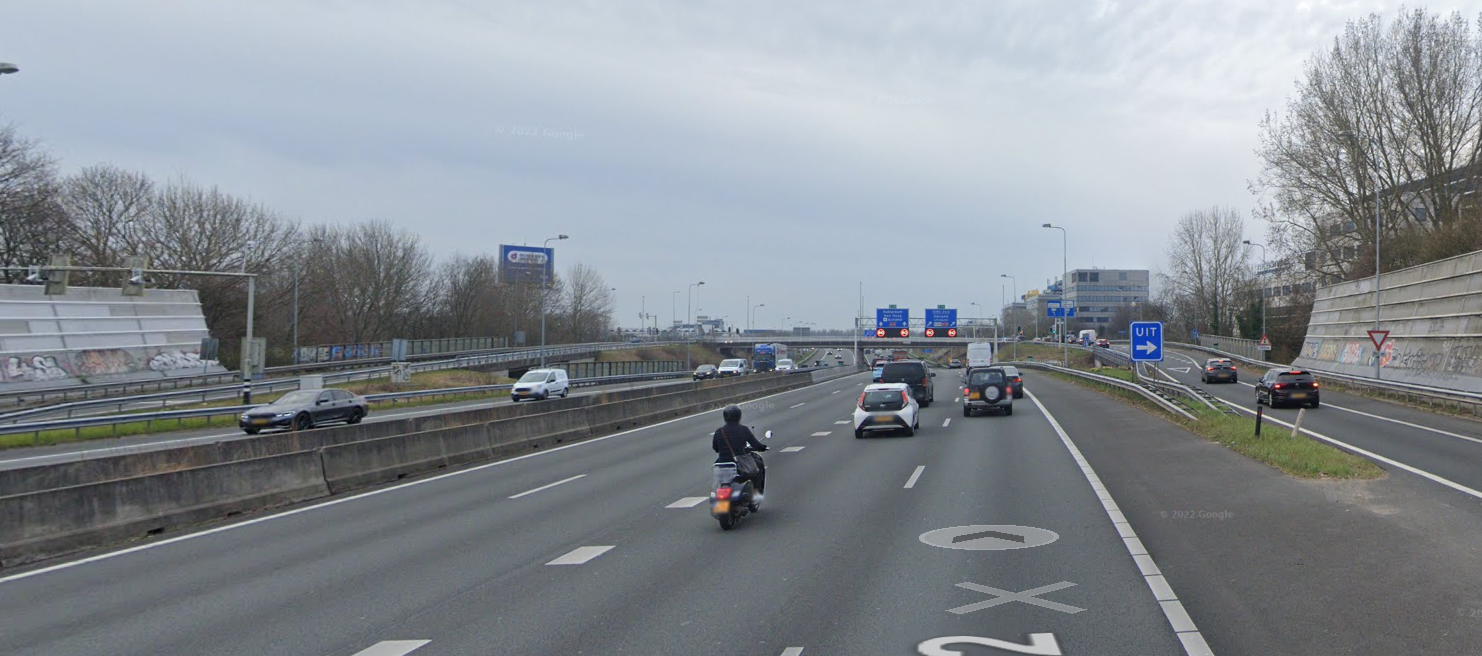
\includegraphics[width = \textwidth]{Amsterdam road.PNG}
    \end{frame}

    \begin{frame}{Einsteinweg, Amsterdam}
        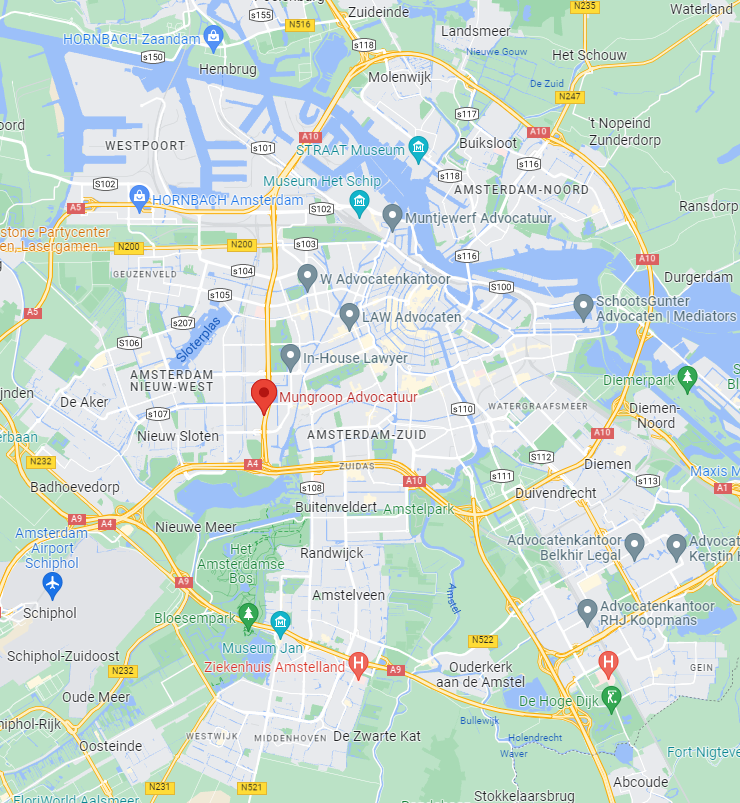
\includegraphics[width = 0.8\textheight]{Amsterdam road map.PNG}
    \end{frame}

    \begin{frame}{Ferdinand Bolstraat, Amsterdam}
        \includegraphics[width = \textwidth]{Amsterdam street.PNG}
    \end{frame}

    \begin{frame}{Sustainable Safety functionality principle}
        \begin{block}{}
            This principle starts from the premise that roads can only have a single function (monofunctionality) and that they must be used in keeping with that function.
            The road function:\\
            \begin{itemize}
                \item \textbf{Through roads} facilitate traffic flow
                \item \textbf{Access roads} provide access to destinations
            \end{itemize}
        \end{block}
        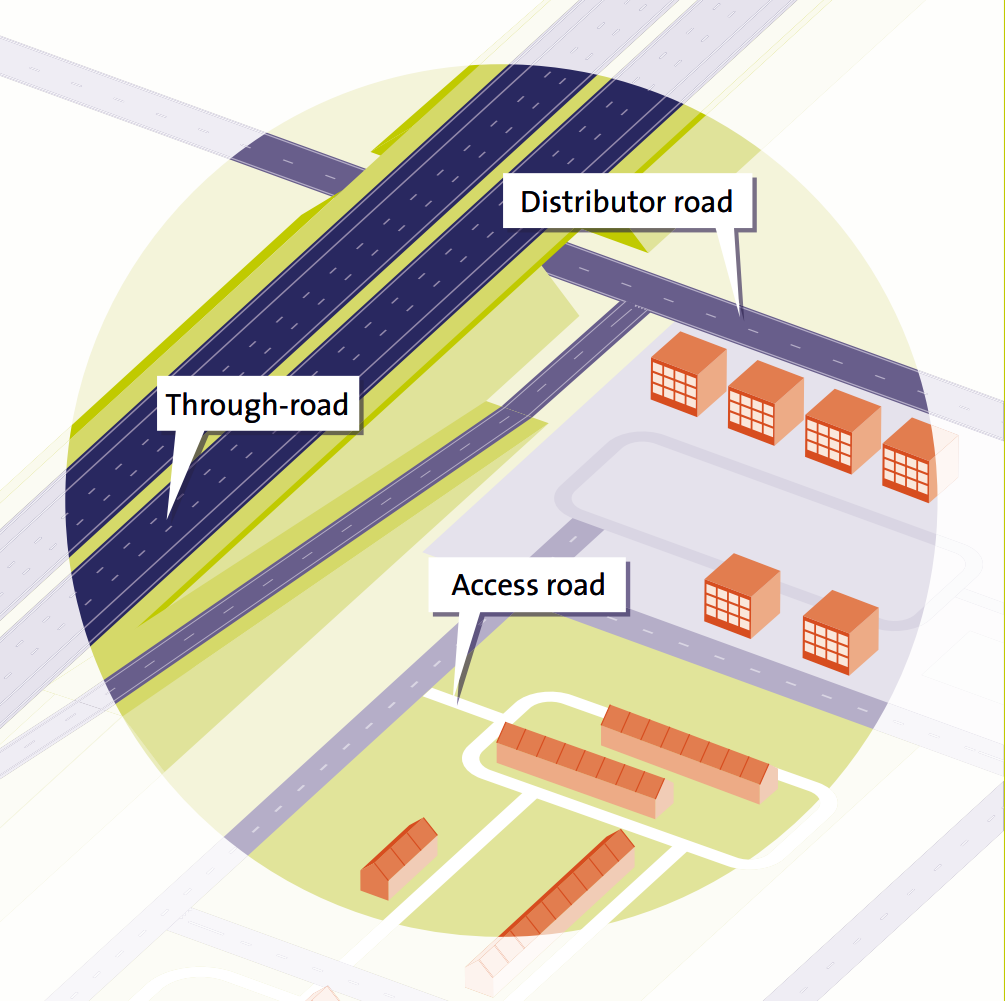
\includegraphics[width = 0.5\textwidth]{Road classification.PNG}
    \end{frame}

    \begin{frame}{Stroad}
        \begin{block}{}
            Does traffic light belongs to street or road?
        \end{block}
    \end{frame}

    \begin{frame}{Sources}
        \begin{block}
            <+->{}
            \begin{itemize}
                \item https://www.youtube.com/watch?v=ORzNZUeUHAM
                \item Sustainable Safety 3rd edition – The advanced vision for 2018-2030
                \item Advancing Sustainable Safety. National Road Safety Outlook for 2005-2020
            \end{itemize}
        \end{block}
    \end{frame}
\end{document}
